
\hypertarget{working_marks}{}
\section{Working with marks}
\index{marks}

\begin{figure}[H]
  \begin{center}
    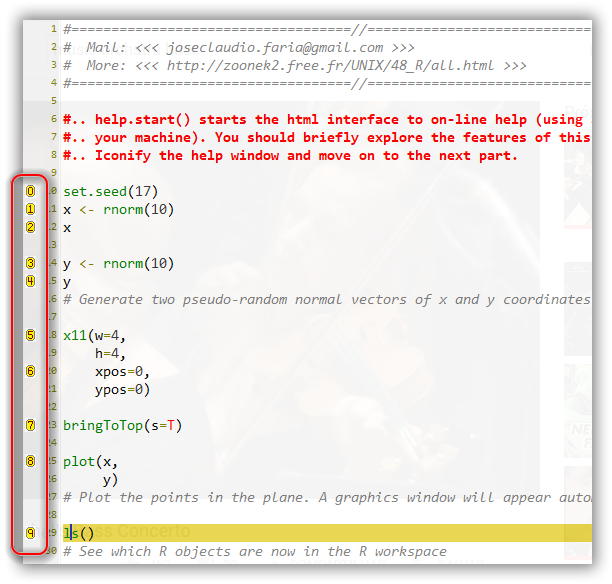
\includegraphics[scale=0.80]{./res/marks.png}
  \end{center}
  \caption{Tinn-R: Marks.}
  \label{fig:tinn-r_marks}
\end{figure}

\subsection{Overview}
When working with long text or program files, moving from one part of the file to another can
be done with the scroll bars, the GoTo line number function (\texttt{CTRL+G}), or under \texttt{Search},
or by searching for specific text strings (\texttt{CTRL+F}).
However, these methods become laborious for frequent moves.
Placing marks in the text at points you will want to return is more efficient.
Marks are visible as small, circled numbers in the left-side column of the editor,
at the start of the line that is marked (Figure \ref{fig:tinn-r_marks}).

Use marks as follows:
\begin{enumerate}
  \item Insert a new mark at the cursor position: \texttt{CTRL + SHIFT + 1 + \ldots + 9}.
    This allows up to 9 separate marks to be inserted
  \item Go to a mark from somewhere else in the text: \texttt{CTRL + 1 + \ldots + 9}.
    Translocation is immediate
  \item Move a mark from one location to another: eg. for Mark 5.
    Position the cursor at the new position, then \texttt{CTRL+SHIFT+5}, as in (1).
    The original position of Mark 5 is lost, and the new position stored.
  \item Delete a mark: position the cursor at the existing position using, eg. \texttt{CTRL+5}.
    Then re-mark 5, as in (1), with \texttt{CTRL+SHIFT+5}
    The number 5 beginning of the line disappears to show that mark 5 has been lost and is free for use later.
\end{enumerate}

Basic options are also available in the \texttt{Misc taskbar} and in the main menu Marks.